\bichapter{模板使用说明}{Template Usage Instructions}
\label{chap:3}

\bisection{图}{Figures}

图片通常在 \texttt{figure} 环境中使用 \texttt{includegraphics} 插入。
建议矢量图片使用 PDF 格式,比如数据可视化的绘图;
照片应使用 JPG 格式;
其他的栅格图应使用无损的 PNG 格式。
注意,LaTeX 不支持 TIFF 格式;EPS 格式已经过时。

\begin{figure}[htbp]
\centering
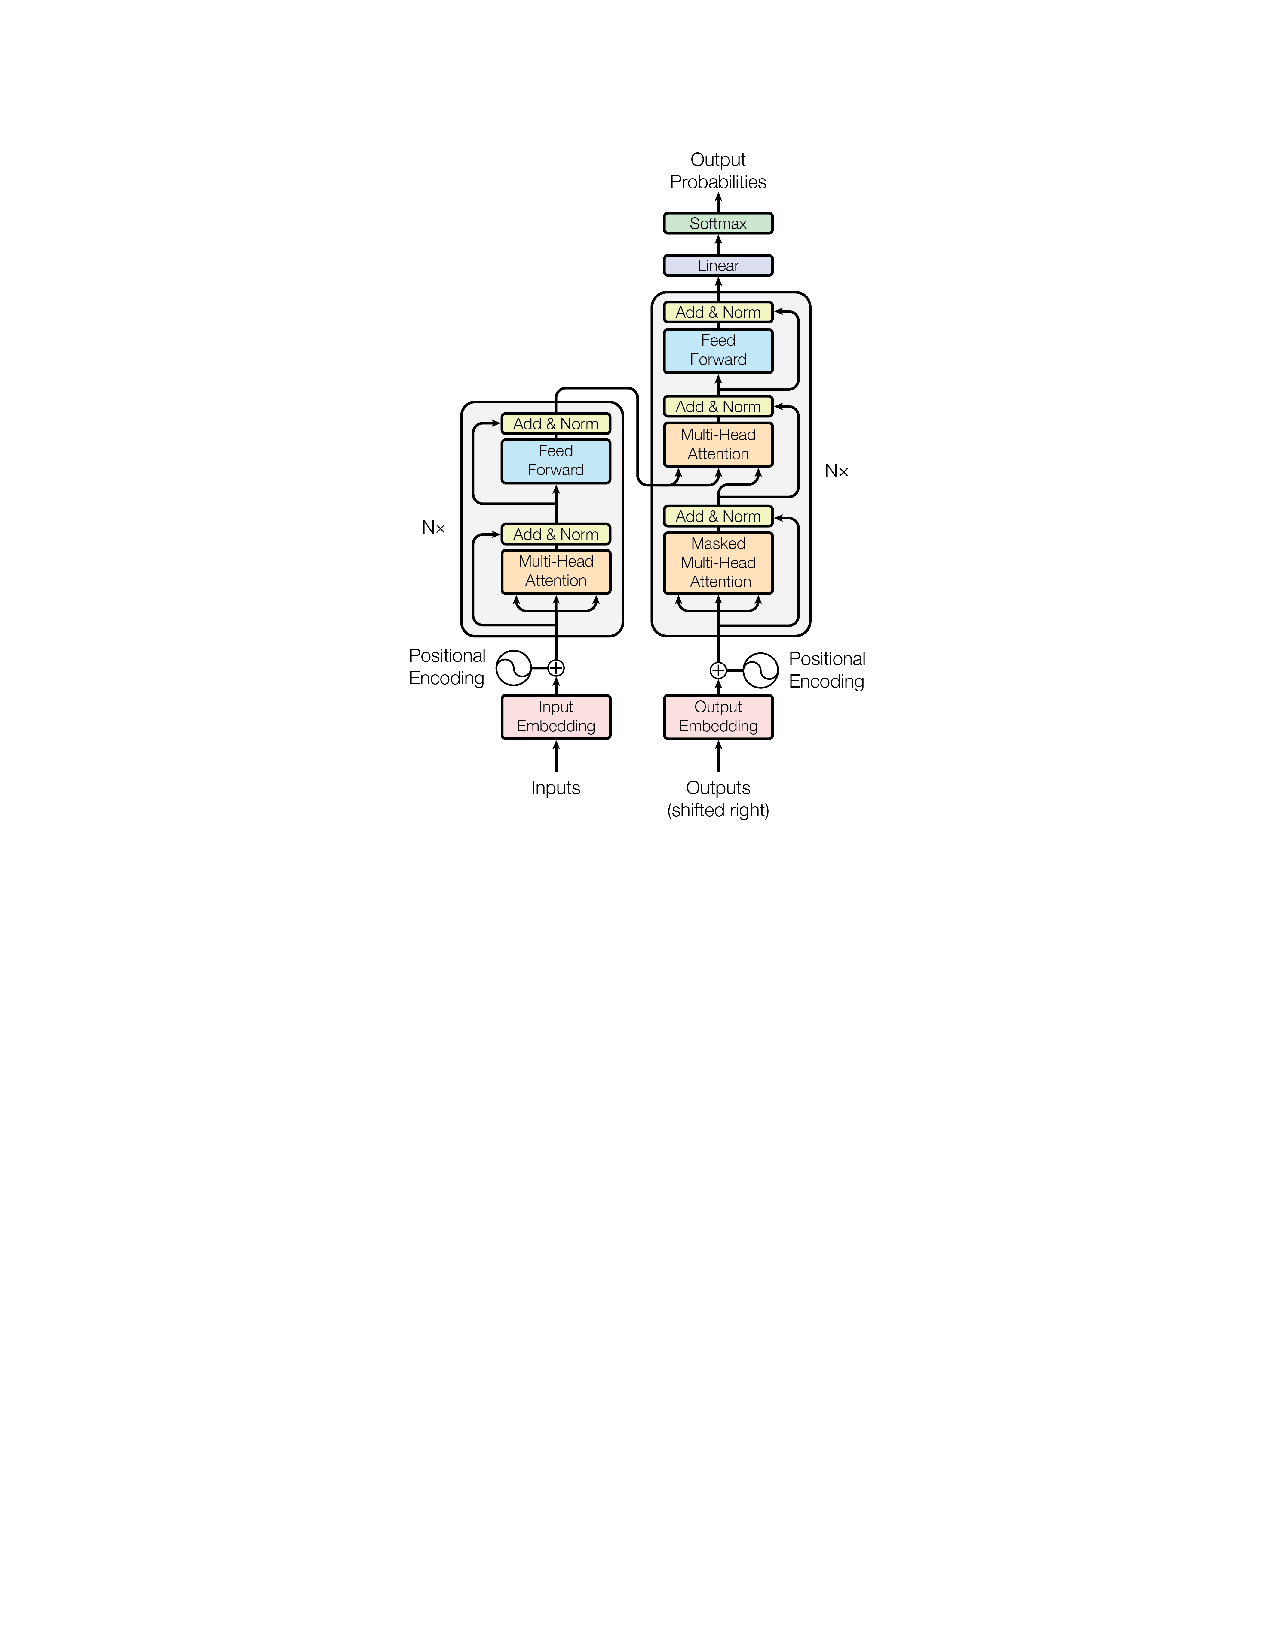
\includegraphics[width=0.55\textwidth]{figures/transformer.pdf}
\bicaption{Transformer模型架构\cite{vaswani2017attention}}{The Transformer - model architecture\cite{vaswani2017attention}}
\label{fig:transformer}
\end{figure}

\begin{figure}[!t]
\centering
\subcaptionbox{HOG + SVM\label{fig:meme:yes}}
    {
\includegraphics[width=0.25\linewidth]{figures/yes.jpg}}
\subcaptionbox{Neural Network\label{fig:meme:no}}
    {
\includegraphics[width=0.25\linewidth]{figures/no.jpg}}
\bicaption{多个分图的示例}{Multiple Sub-Figures}
\label{fig:meme}
\end{figure}

若图或表中有附注,采用英文小写字母顺序编号,附注写在图或表的下方。
国外的期刊习惯将图表的标题和说明文字写成一段,需要改写为标题只含图表的名称,其他说明文字以注释方式写在图表下方,或者写在正文中。

如果一个图由两个或两个以上分图组成时,各分图分别以 (a)、(b)、(c)...... 作为图序,并须有分图标题。
推荐使用 \texttt{subcaption} 宏包来处理, 比如图~\ref{fig:meme:yes} 和图~\ref{fig:meme:no}。


\bisection{表}{Tables}

表应具有自明性。为使表格简洁易读,尽可能采用三线表,如表~\ref{tab:datasets}。
三条线可以使用 \texttt{booktabs} 宏包提供的命令生成。

\begin{table}[htbp]
\small
\centering
\bicaption{数据集概览}{Summary of Datasets}
\begin{tabular}{lcccccc}
\toprule
数据集 & 样本数量 & 记录数量 & 特征数量 & 平均记录数量 & 类别数 & $p/r$\\
\midrule
PPMI & 683 & 15798 & 212 & 23.1303 & 2 & 9/1 \\
PS & 68 & 1208 & 26 & 17.7647 & 2 & 1.5/1 \\
OD & 115 & 20560 & 5 & 178.7826 & 2 & 1/36 \\
\bottomrule
\end{tabular}
\label{tab:datasets}
\end{table}


\bisection{算法}{Algorithms}

算法环境可以使用 \texttt{algorithms} 宏包。

\begin{algorithm}[htbp]
\caption{算法示例}
\label{alg:cram_mult}
\begin{algorithmic}[1]
\State $i \gets 10$
\If{$i\geq 5$} 
    \State $i \gets i-1$
\Else
    \If{$i\leq 3$}
        \State $i \gets i+2$
    \EndIf
\EndIf
\end{algorithmic}
\end{algorithm}